% Created by tikzDevice version 0.12.3 on 2020-02-06 15:34:25
% !TEX encoding = UTF-8 Unicode
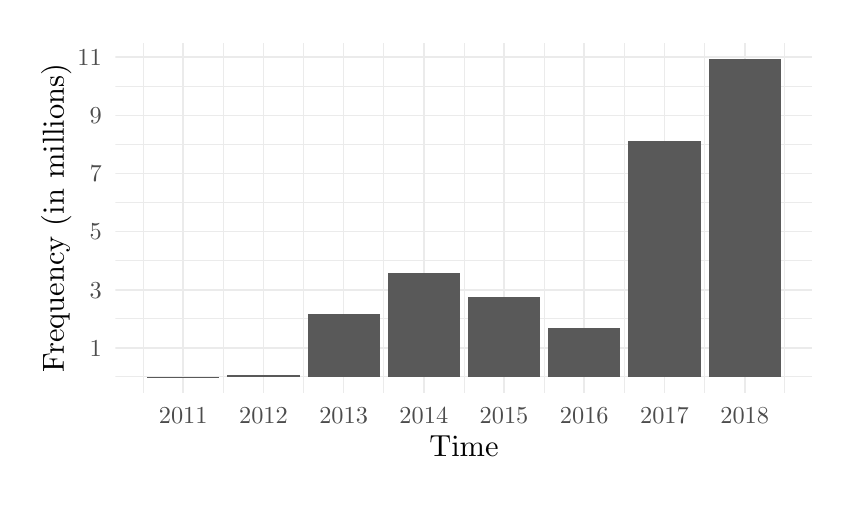
\begin{tikzpicture}[x=1pt,y=1pt]
\definecolor{fillColor}{RGB}{255,255,255}
\path[use as bounding box,fill=fillColor,fill opacity=0.00] (0,0) rectangle (289.08,162.61);
\begin{scope}
\path[clip] ( 31.71, 30.69) rectangle (283.58,157.11);
\definecolor{drawColor}{gray}{0.92}

\path[draw=drawColor,line width= 0.3pt,line join=round] ( 31.71, 36.43) --
	(283.58, 36.43);

\path[draw=drawColor,line width= 0.3pt,line join=round] ( 31.71, 57.43) --
	(283.58, 57.43);

\path[draw=drawColor,line width= 0.3pt,line join=round] ( 31.71, 78.42) --
	(283.58, 78.42);

\path[draw=drawColor,line width= 0.3pt,line join=round] ( 31.71, 99.41) --
	(283.58, 99.41);

\path[draw=drawColor,line width= 0.3pt,line join=round] ( 31.71,120.41) --
	(283.58,120.41);

\path[draw=drawColor,line width= 0.3pt,line join=round] ( 31.71,141.40) --
	(283.58,141.40);

\path[draw=drawColor,line width= 0.3pt,line join=round] ( 41.71, 30.69) --
	( 41.71,157.11);

\path[draw=drawColor,line width= 0.3pt,line join=round] ( 70.70, 30.69) --
	( 70.70,157.11);

\path[draw=drawColor,line width= 0.3pt,line join=round] ( 99.68, 30.69) --
	( 99.68,157.11);

\path[draw=drawColor,line width= 0.3pt,line join=round] (128.66, 30.69) --
	(128.66,157.11);

\path[draw=drawColor,line width= 0.3pt,line join=round] (157.65, 30.69) --
	(157.65,157.11);

\path[draw=drawColor,line width= 0.3pt,line join=round] (186.63, 30.69) --
	(186.63,157.11);

\path[draw=drawColor,line width= 0.3pt,line join=round] (215.61, 30.69) --
	(215.61,157.11);

\path[draw=drawColor,line width= 0.3pt,line join=round] (244.60, 30.69) --
	(244.60,157.11);

\path[draw=drawColor,line width= 0.3pt,line join=round] (273.58, 30.69) --
	(273.58,157.11);

\path[draw=drawColor,line width= 0.6pt,line join=round] ( 31.71, 46.93) --
	(283.58, 46.93);

\path[draw=drawColor,line width= 0.6pt,line join=round] ( 31.71, 67.92) --
	(283.58, 67.92);

\path[draw=drawColor,line width= 0.6pt,line join=round] ( 31.71, 88.92) --
	(283.58, 88.92);

\path[draw=drawColor,line width= 0.6pt,line join=round] ( 31.71,109.91) --
	(283.58,109.91);

\path[draw=drawColor,line width= 0.6pt,line join=round] ( 31.71,130.90) --
	(283.58,130.90);

\path[draw=drawColor,line width= 0.6pt,line join=round] ( 31.71,151.90) --
	(283.58,151.90);

\path[draw=drawColor,line width= 0.6pt,line join=round] ( 56.20, 30.69) --
	( 56.20,157.11);

\path[draw=drawColor,line width= 0.6pt,line join=round] ( 85.19, 30.69) --
	( 85.19,157.11);

\path[draw=drawColor,line width= 0.6pt,line join=round] (114.17, 30.69) --
	(114.17,157.11);

\path[draw=drawColor,line width= 0.6pt,line join=round] (143.15, 30.69) --
	(143.15,157.11);

\path[draw=drawColor,line width= 0.6pt,line join=round] (172.14, 30.69) --
	(172.14,157.11);

\path[draw=drawColor,line width= 0.6pt,line join=round] (201.12, 30.69) --
	(201.12,157.11);

\path[draw=drawColor,line width= 0.6pt,line join=round] (230.11, 30.69) --
	(230.11,157.11);

\path[draw=drawColor,line width= 0.6pt,line join=round] (259.09, 30.69) --
	(259.09,157.11);
\definecolor{fillColor}{gray}{0.35}

\path[fill=fillColor] ( 43.16, 36.43) rectangle ( 69.25, 36.44);

\path[fill=fillColor] ( 72.14, 36.43) rectangle ( 98.23, 37.20);

\path[fill=fillColor] (101.13, 36.43) rectangle (127.21, 58.99);

\path[fill=fillColor] (130.11, 36.43) rectangle (156.20, 74.09);

\path[fill=fillColor] (159.10, 36.43) rectangle (185.18, 65.17);

\path[fill=fillColor] (188.08, 36.43) rectangle (214.16, 54.20);

\path[fill=fillColor] (217.06, 36.43) rectangle (243.15,121.65);

\path[fill=fillColor] (246.05, 36.43) rectangle (272.13,151.36);
\end{scope}
\begin{scope}
\path[clip] (  0.00,  0.00) rectangle (289.08,162.61);
\definecolor{drawColor}{gray}{0.30}

\node[text=drawColor,anchor=base east,inner sep=0pt, outer sep=0pt, scale=  0.88] at ( 26.76, 43.90) {1};

\node[text=drawColor,anchor=base east,inner sep=0pt, outer sep=0pt, scale=  0.88] at ( 26.76, 64.89) {3};

\node[text=drawColor,anchor=base east,inner sep=0pt, outer sep=0pt, scale=  0.88] at ( 26.76, 85.89) {5};

\node[text=drawColor,anchor=base east,inner sep=0pt, outer sep=0pt, scale=  0.88] at ( 26.76,106.88) {7};

\node[text=drawColor,anchor=base east,inner sep=0pt, outer sep=0pt, scale=  0.88] at ( 26.76,127.87) {9};

\node[text=drawColor,anchor=base east,inner sep=0pt, outer sep=0pt, scale=  0.88] at ( 26.76,148.87) {11};
\end{scope}
\begin{scope}
\path[clip] (  0.00,  0.00) rectangle (289.08,162.61);
\definecolor{drawColor}{gray}{0.30}

\node[text=drawColor,anchor=base,inner sep=0pt, outer sep=0pt, scale=  0.88] at ( 56.20, 19.68) {2011};

\node[text=drawColor,anchor=base,inner sep=0pt, outer sep=0pt, scale=  0.88] at ( 85.19, 19.68) {2012};

\node[text=drawColor,anchor=base,inner sep=0pt, outer sep=0pt, scale=  0.88] at (114.17, 19.68) {2013};

\node[text=drawColor,anchor=base,inner sep=0pt, outer sep=0pt, scale=  0.88] at (143.15, 19.68) {2014};

\node[text=drawColor,anchor=base,inner sep=0pt, outer sep=0pt, scale=  0.88] at (172.14, 19.68) {2015};

\node[text=drawColor,anchor=base,inner sep=0pt, outer sep=0pt, scale=  0.88] at (201.12, 19.68) {2016};

\node[text=drawColor,anchor=base,inner sep=0pt, outer sep=0pt, scale=  0.88] at (230.11, 19.68) {2017};

\node[text=drawColor,anchor=base,inner sep=0pt, outer sep=0pt, scale=  0.88] at (259.09, 19.68) {2018};
\end{scope}
\begin{scope}
\path[clip] (  0.00,  0.00) rectangle (289.08,162.61);
\definecolor{drawColor}{RGB}{0,0,0}

\node[text=drawColor,anchor=base,inner sep=0pt, outer sep=0pt, scale=  1.10] at (157.65,  7.64) {Time};
\end{scope}
\begin{scope}
\path[clip] (  0.00,  0.00) rectangle (289.08,162.61);
\definecolor{drawColor}{RGB}{0,0,0}

\node[text=drawColor,rotate= 90.00,anchor=base,inner sep=0pt, outer sep=0pt, scale=  1.10] at ( 13.08, 93.90) {Frequency (in millions)};
\end{scope}
\end{tikzpicture}
